% interactcadsample.tex
% v1.03 - April 2017

\documentclass[]{interact}

\usepackage{epstopdf}% To incorporate .eps illustrations using PDFLaTeX, etc.
\usepackage{subfigure}% Support for small, `sub' figures and tables
%\usepackage[nolists,tablesfirst]{endfloat}% To `separate' figures and tables from text if required

\usepackage{natbib}% Citation support using natbib.sty
\bibpunct[, ]{(}{)}{;}{a}{}{,}% Citation support using natbib.sty
\renewcommand\bibfont{\fontsize{10}{12}\selectfont}% Bibliography support using natbib.sty

\theoremstyle{plain}% Theorem-like structures provided by amsthm.sty
\newtheorem{theorem}{Theorem}[section]
\newtheorem{lemma}[theorem]{Lemma}
\newtheorem{corollary}[theorem]{Corollary}
\newtheorem{proposition}[theorem]{Proposition}

\theoremstyle{definition}
\newtheorem{definition}[theorem]{Definition}
\newtheorem{example}[theorem]{Example}

\theoremstyle{remark}
\newtheorem{remark}{Remark}
\newtheorem{notation}{Notation}


% tightlist command for lists without linebreak
\providecommand{\tightlist}{%
  \setlength{\itemsep}{0pt}\setlength{\parskip}{0pt}}



\usepackage{lscape}
\usepackage{hyperref}
\usepackage[utf8]{inputenc}
\def\tightlist{}
\usepackage{setspace}
\doublespacing

\usepackage{booktabs}
\usepackage{longtable}
\usepackage{array}
\usepackage{multirow}
\usepackage{wrapfig}
\usepackage{float}
\usepackage{colortbl}
\usepackage{pdflscape}
\usepackage{tabu}
\usepackage{threeparttable}
\usepackage{threeparttablex}
\usepackage[normalem]{ulem}
\usepackage{makecell}
\usepackage{xcolor}

\begin{document}


\articletype{ARTICLE TEMPLATE}

\title{Automated reading of residual plots with computer vision models}


\author{\name{Weihao Li$^{a}$}
\affil{$^{a}$Department of Econometrics and Business Statistics, Monash
University, Clayton, VIC, Australia}
}

\thanks{CONTACT Weihao
Li. Email: \href{mailto:weihao.li@monash.edu}{\nolinkurl{weihao.li@monash.edu}}}

\maketitle

\begin{abstract}
TBD.
\end{abstract}

\begin{keywords}
TBD
\end{keywords}

\newpage
\tableofcontents
\newpage

\hypertarget{introduction}{%
\section{Introduction}\label{introduction}}

The practice of plotting residuals is commonly regarded as a standard
procedure in linear regression diagnostics
\citep[see][]{cook1982residuals, belsley1980regression}. This visual
assessment plays a crucial role in identifying deviations from model
assumptions, such as linearity, homoscedasticity, and normality. It also
helps in understanding the goodness of fit and various characteristics
of the model.

Generating a residual plot in most statistical software is often as
straightforward as executing a line of code or clicking a button.
However, accurately interpreting a residual plot can be challenging.
Consider Figure \ref{fig:false-finding} as an example, the residuals
display a triangular shape pointing to the left. While this might
suggest heteroskedasticity, it is important to avoid over-interpreting
the visual pattern. In this case, the fitted model is correctly
specified, and the triangular shape is actually a result of the skewed
distribution of the predictors, rather than indicating a flaw in the
model.

A residual plot can exhibit various visual features, but it is crucial
to recognize that some may arise from the characteristics of predictors
and the inherent randomness of the error, rather than indicating a
violation of model assumptions \citep{li2023plot}. The concept of visual
inference, as proposed by \citet{buja2009statistical}, provides an
inferential framework to assess whether residual plots indeed contain
visual patterns inconsistent with the model assumptions. The fundamental
idea involves testing whether the actual residual plot visually differs
significantly from null plots, which are created using residuals
generated from the null distribution. Typically, this is accomplished
through the lineup protocol. In this approach, the real residual plot is
embedded within a lineup alongside several null plots. If the real
residual plot can be distinguished from the lineup, it provides evidence
for rejecting the null hypothesis.

The practice of delivering a residual plot as a lineup is generally
regarded as a valuable approach. Beyond its application in residual
diagnostics, the lineup protocol has integrated into the analysis of
diverse subjects. For instance,
\cite{loy2013diagnostic, loy2014hlmdiag, loy2015you} illustrate its
applicability in diagnosing hierarchical linear models. Additionally,
\citet{widen2016graphical} demonstrates its utility in geographical
research, while \citet{krishnan2021hierarchical} explores its
effectiveness in forensic examinations.

However, as pointed out by \citet{li2023plot}, a primary limitation of
the lineup protocol lies in its reliance on human judgments. Unlike
conventional statistical tests that can be performed numerically and
automatically in statistical software, the lineup protocol requires
human evaluation of images. This characteristic makes it less suitable
for large-scale applications, given the associated high labor costs and
time requirements.

There is a substantial need to develop an approach that alleviates
people's workload by automating repetitive tasks and providing
standardized results in a controlled environment. The large-scale
evaluation of lineups is impractical without the use of technology and
machines.

The utilization of computers to interpret data plots has a rich history,
with early efforts such as ``Scagnostics'' by \citet{tukey1985computer},
focusing on scatterplot diagnostics. \citet{wilkinson2005graph} expanded
on this work, introducing graph theoretic scagnostics, which encompassed
nine computable measures applied to planar proximity graphs. These
measures, including, but not limited to, ``Outlying'', ``Skinny'',
``Stringy'', ``Straight'', ``Monotonic'', ``Skewed'', ``Clumpy'', and
``Striated'' aimed to characterize outliers, shape, density, trend,
coherence and other characteristics of the data. While this approach has
been inspiring, there is a recognition \citep{buja2009statistical} that
it may not capture all the necessary visual features that differentiate
actual residual plots from null plots. A more promising alternative
entails enabling computers to learn the function for extracting visual
features from residual plots. Essentially, this means empowering
computers to discern the crucial visual features for residual
diagnostics and determining the method to extract them. Modern computer
vision models are well-suited for addressing this challenge.

Modern computer vision models often rely on deep neural networks with
convolutional layers \citep{fukushima1982neocognitron}. These layers
leverage hierarchical patterns in data, downsizing and transforming
images by summarizing information in a small space. Numerous studies
have demonstrated the efficacy of convolutional layers in addressing
various vision tasks, including image recognition \citep{rawat2017deep}.
Despite the widespread use of computer vision models in fields like
computer-aided diagnosis \citep{lee2015image}, pedestrian detection
\citep{brunetti2018computer}, and facial recognition
\citep{emami2012facial}, their application in reading data plots remains
limited. While some studies have explored the use of computer vision
models for tasks such as reading recurrence plots for time series
regression \citep{ojeda2020multivariate}, time series classification
\citep{chu2019automatic, hailesilassie2019financial, hatami2018classification, zhang2020encoding},
anomaly detection \citep{chen2020convolutional}, and pairwise causality
analysis \citep{singh2017deep}, the application of reading residual
plots with computer vision models represents a relatively new field of
study.

In this paper, we develop computer vision models and integrate them into
the residual plots diagnostics workflow, filling the gap of\ldots. The
paper is structured as follows: \ldots{}

\begin{figure}

{\centering 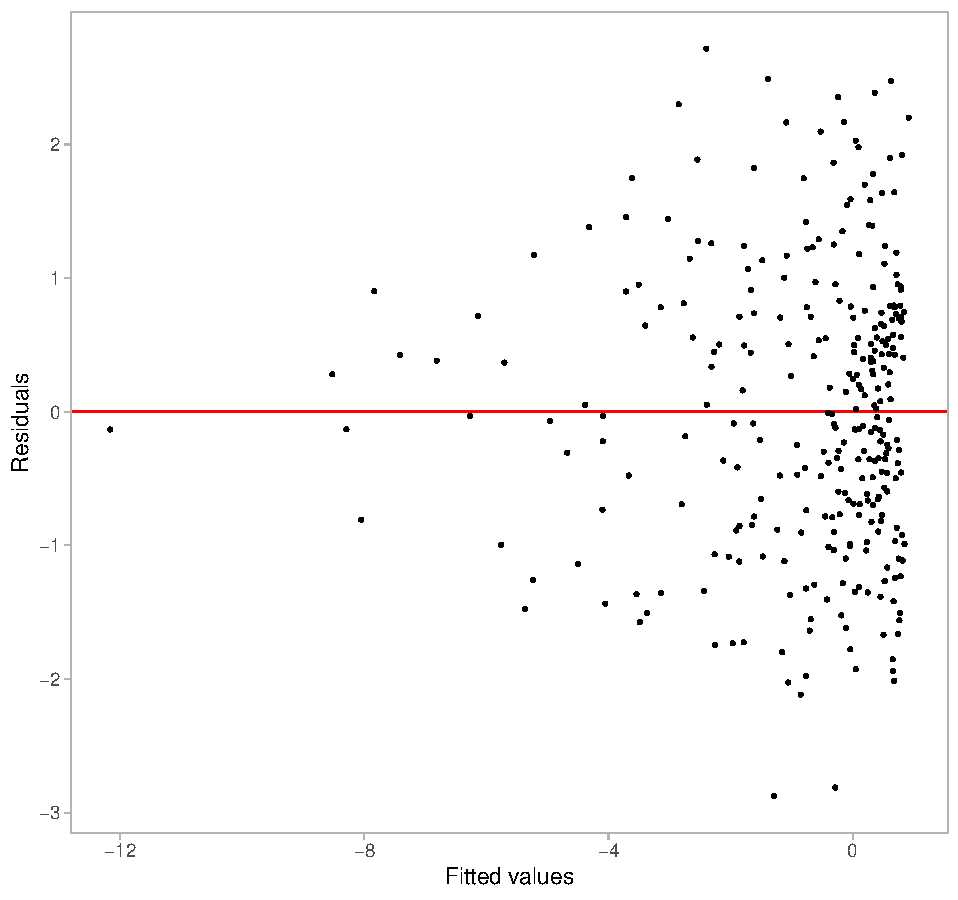
\includegraphics[width=1\linewidth]{paper_files/figure-latex/false-finding-1} 

}

\caption{An example residual vs fitted values plot (red line indicates 0). The vertical spread of the data points varies with the fitted values. This often indicates the existence of heteroskedasticity.}\label{fig:false-finding}
\end{figure}

\hypertarget{methodology}{%
\section{Methodology}\label{methodology}}

\hypertarget{different-possible-configurations-of-the-model-formula}{%
\subsection{Different possible configurations of the model
formula}\label{different-possible-configurations-of-the-model-formula}}

In addressing the residual reading problem, there exist multiple
configurations of the computer vision model formula. These
configurations can be categorized by two key components of the model
formula: the input and the output format.

\hypertarget{different-input-formats}{%
\subsubsection{Different input formats}\label{different-input-formats}}

In computer vision models, the quality and relevance of the input data
greatly influence the model's capacity to generate insightful and
meaningful results. The input of the model can be designed in different
formats.

A straightforward approach involves feeding the model a vector of
residuals along with a vector of fitted values, essentially providing
all the necessary information for creating a residuals vs fitted values
plot. However, a drawback of this method is the dynamic input size, as
different fitted regression models may have varying numbers of
observations. For modern computer vision models implemented with
mainstream software like TensorFlow \citep{abadi2016tensorflow}, the
input shape is typically fixed. One solution is to pad the input vectors
with leading or trailing zeros if the input tensor expects longer
vectors, but it may fail if the input vector surpasses the designed
length. Another strategy is to summarize the residuals and fitted values
separately using histograms and utilize the counts as the input. By
controlling the number of bins in the histograms, it becomes possible to
provide fixed-length input vectors.

Another approach is to use an image as input. The primary advantage of
using an image, as opposed to the vector format, is the utilization of
the sophisticated image processing architectures developed over the
years, such as the VGG16 architecture proposed in
\citet{simonyan2014very}. These architectures can effectively capture
and summarize spatial information from nearby pixels, which is less
straightforward with vector input. The only considerations are the image
resolution and the aesthetics of the residual plot. In general, higher
resolution provides more information to the model but comes with the
trade-off of increased complexity and greater difficulty in training. As
for the aesthetics of the residual plot, a practical solution is to
consistently present residual plots in the same style to the model. This
implies that the model can not accept arbitrary images as input but
requires the use of the same preprocessing software to convert provided
residuals and fitted values into a standardized style for the residual
plot.

Other possible input formats include, but are not limited to, a pair of
residual plots, a triplet, and a lineup. \citet{chopra2005learning} has
shown that computer vision models designed for image comparison can
assess whether a pair of images are similar or dissimilar. Applied to
our specific problem, we can define null plots of a fitted model to be
similar to each other, while considering actual residual plots to be
distinct from null plots of any fitted model. A triplet constitutes a
set of three images, denoted as \(image_1\), \(image_2\) and
\(image_3\). It is often used to predict whether \(image_2\) or
\(image_3\) is more similar to \(image_1\), proving particularly useful
for establishing rankings between samples. However, it's important to
note that these two approaches usually require additional considerations
regarding the loss function and, at times, non-standard training
processes due to shared weights between different convolutional blocks.

Presenting a lineup to a model and asking it to predict which residual
plot is the most different one aligns closely with the lineup protocol.
However, if a lineup consists of a large amount of residual plots, the
resolution of the input image could become quite large, posing
challenges in training the model. This approach was experimented in a
pilot study conducted by us but the performance of the trained model was
sub-optimal.

Not all the mentioned input formats were explored and tested in this
study due to the considerable costs associated with data preparation and
model training. The single residual plot input format was chosen for its
relatively low implementation cost and high interpretability.

\hypertarget{different-output-formats}{%
\subsubsection{Different output
formats}\label{different-output-formats}}

Given that the input is a single residual plot represented as a
fixed-resolution image, the computer vision model's output can take one
of two formats: binary or numeric. This choice determines whether the
model belongs to a classification model or a regression model. The
binary outcome might indicates whether the input image is a null plot or
not, or whether the input image would be rejected in a visual test
conducted by humans. The latter option requires data from prior human
subject experiments, presenting difficulties in controlling the quality
of data due to variations in experimental settings across different
studies. Additionally, some visual inference experiments are unrelated
to linear regression models and residual plots, resulting in a limited
amount of available training data.

Alternatively, the output could be a meaningful numeric measure, such as
the average distance to good residual plots. This approach necessitates
defining a distance measure between residual plots, which may be a
non-trivial task. However, once a meaningful distance measure is
established, the computer vision model's prediction becomes an
interpretable value with tangible significance. Studies have
demonstrated that defining a proper distance between images can enhance
the matching accuracy in image search compared to a binary outcome model
(ref here).

\hypertarget{distance-from-the-good-residual-plots}{%
\subsection{Distance from the good residual
plots}\label{distance-from-the-good-residual-plots}}

In a visual test, the observer will be asked to choose one or more plots
that stand out as most distinct from others in a given lineup. To
develop a computer vision model for evaluating residual plots within the
visual inference framework, it is important to precisely define a
numerical measure of ``difference'' or ``distance'' between plots. This
distance can take the form of a basic statistical operation on pixels,
such as the sum of square differences. Alternatively, it could involve
established image similarity metrics like the Structural Similarity
Index Measure \citep{wang2004image}. The challenge lies in the fact that
metrics tailored for image comparison may not be suitable for evaluating
data plots, where only essential plot elements require assessment
\citep{chowdhury2018measuring}. Furthermore, scagnostics mentioned in
Section \ref{introduction} could be used to construct distance metrics
for data plots comparison, but the functional form still needs to be
carefully refined to accurately reflect the extent of the violations.

\hypertarget{residual-distribution}{%
\subsubsection{Residual distribution}\label{residual-distribution}}

The distance metrics proposed in this paper takes into account the fact
that we try to measure how different a residual plot is from a good
residual plot, or in other words, how different a given fitted model is
from a correctly specified model. For the classical normal linear
regression model, residuals are derived from the fitted values
\(\hat{\boldsymbol{y}}\) and observed values \(\boldsymbol{y}\). Suppose
the data generating process is known and the model is correctly
specified, by the Frisch-Waugh-Lowell theorem \citep{frisch1933partial},
residuals \(\boldsymbol{e}\) can also be written as a linear
transformation of the error \(\boldsymbol{\varepsilon}\) formulated as
\(\boldsymbol{e} = \boldsymbol{R}\boldsymbol{\varepsilon}\), where
\(\boldsymbol{R}=\boldsymbol{I}_n -\boldsymbol{X}(\boldsymbol{X}'\boldsymbol{X})^{-1}\boldsymbol{X}'\)
is the residual operator, \(\boldsymbol{X}\) is the design matrix,
\(\boldsymbol{I}_n\) is a \(n\) by \(n\) identity matrix, and \(n\) is
the number of observations.

One of the assumptions of the classical normal linear regression model
is the error \(\boldsymbol{\varepsilon}\) follows a multivariate normal
distribution with zero mean and constant variance, i.e.,
\(\boldsymbol{\varepsilon} \sim N(\boldsymbol{0}_n,\sigma^2\boldsymbol{I}_n)\).
It can be known that residuals \(\boldsymbol{e}\) also follow a certain
probability distribution transformed from the multivariate normal
distribution, which will be denoted as \(Q\). This reference
distribution \(Q\) summarizes what good residuals should follow given
the predictors are known and fixed.

When fitting a linear regression model, the solver will force
\(\sum_{i=1}^{n} e_i = 0\), making any residual value to be a linear
combination of the remaining \(n - 1\) residuals. This effectively means
\(rank(\boldsymbol{R}) = n - 1 < n\) and \(Q\) becomes a degenerate
multivariate distribution. To capture the characteristics of \(Q\), such
as moments, we can simulate a large numbers of
\(\boldsymbol{\varepsilon}\) and transform it to \(\boldsymbol{e}\) to
get the empirical estimates. For simplicity, we replaced
\(\boldsymbol{R}\) with a full-rank diagonal matrix
\(diag(\boldsymbol{R})\), where \(diag(.)\) set the non-diagonal entries
of a matrix to zeros. The resulting distribution for \(\boldsymbol{Q}\)
is \(N(\boldsymbol{0}_n, diag(\boldsymbol{R}\sigma^2))\).

Distribution \(Q\) is derived from the correctly specified model.
However, if the model is misspecified, then the actual distribution of
residuals denoted as \(P\), will be different to \(Q\). For example, if
the data generating process contains variables correlated with any
column of \(\boldsymbol{X}\) but not included in \(\boldsymbol{X}\),
causing an omitted variable problem, \(P\) will be different to \(Q\)
because the residual operator obtained from the fitted model will not be
the same as \(\boldsymbol{R}\). Besides, if the
\(\boldsymbol{\varepsilon}\) follows a non-normal distribution such as a
multivariate lognormal distribution, the empirical residual distribution
will usually be skewed and has a long tail.

\hypertarget{kullback-leibler-divergence-of-p-from-q}{%
\subsubsection{\texorpdfstring{Kullback-Leibler divergence of \(P\) from
\(Q\)}{Kullback-Leibler divergence of P from Q}}\label{kullback-leibler-divergence-of-p-from-q}}

Define a proper distance between distributions is usually easier than
define a proper distance between data plots. Given the actual residual
distribution \(Q\) and the reference residual distribution \(P\), we
used a distance metric based on Kullback-Leibler divergence
\citep{kullback1951information} to quantify the difference between two
distributions

\begin{align}
\label{eq:kl-0}
D &= log\left(1 + D_{KL}\right), \\
\label{eq:kl-1}
D_{KL} &= \int_{\mathbb{R}^{n}}log\frac{p(\boldsymbol{e})}{q(\boldsymbol{e})}p(\boldsymbol{e})d\boldsymbol{e},
\end{align}

\noindent where \(p(.)\) is the probability density function for
distribution \(P\), and \(q(.)\) is the probability density function for
distribution \(Q\).

This distance metric was first proposed in \citet{li2023plot}. It was
mainly designed for measuring the effect size of non-linearity and
heteroskedasticity in a residual plot. \citet{li2023plot} showed that,
for a classical normal linear regression model that omits a necessary
higher-order predictors \(\boldsymbol{Z}\), and incorrectly assumes
\(\boldsymbol{\varepsilon} \sim N(\boldsymbol{0}_n,\sigma^2\boldsymbol{I}_n)\)
while in fact
\(\boldsymbol{\varepsilon} \sim N(\boldsymbol{0}_n, \boldsymbol{V})\),
\(Q\) can be represented as
\(N(\boldsymbol{R}\boldsymbol{Z}\boldsymbol{\beta}_z, diag(\boldsymbol{R}\boldsymbol{V}\boldsymbol{R}'))\).
Note that the variance-covariance matrix is replaced with the diagonal
matrix to ensure it is a full-rank matrix.

Since both \(P\) and \(Q\) are adjusted to be multivariate normal
distributions, equation \ref{eq:kl-1} can be further expanded to

\begin{align}
\label{eq:kl-2}
D_{KL} &= \frac{1}{2}\left(\log\frac{|\text{diag}(\boldsymbol{W})|}{|\text{diag}(\boldsymbol{R}\sigma^2)|} - n + \text{tr}(\text{diag}(\boldsymbol{W})^{-1}\text{diag}(\boldsymbol{R}\sigma^2)) + \boldsymbol{\mu}_z'(diag(\boldsymbol{W}))^{-1}\boldsymbol{\mu}_z\right),
\end{align}

\noindent where
\(\boldsymbol{\mu}_z = \boldsymbol{R}\boldsymbol{Z}\boldsymbol{\beta}_z\),
and \(\boldsymbol{W} = \boldsymbol{R}\boldsymbol{V}\boldsymbol{R}'\).
The assumed error variance \(\sigma^2\) is set to be
\(tr(\boldsymbol{V})/n\), which is the expectation of the estimated
variance.

\hypertarget{evaluation-of-kullback-leibler-divergence-for-non-normal-p}{%
\subsubsection{\texorpdfstring{Evaluation of Kullback-Leibler divergence
for non-normal
\(P\)}{Evaluation of Kullback-Leibler divergence for non-normal P}}\label{evaluation-of-kullback-leibler-divergence-for-non-normal-p}}

For non-normal error \(\boldsymbol{\varepsilon}\), the actual residual
distribution \(P\) is unlikely to be a multivariate normal distribution.
Thus, equation \ref{eq:kl-2} given in \citet{li2023plot} will not be
applicable to models with non-normality violations.

To evaluate the Kullback-Leibler divergence of non-normal \(P\) from
\(Q\), the fallback is to solve equation \ref{eq:kl-1} numerically.
However, since \(\boldsymbol{e}\) is a linear transformation of
non-normal random variables, it is very common that the general form of
\(P\) is unknown, meaning that we can not easily compute
\(p(\boldsymbol{e})\) using a well-known probability density function.
Additionally, even if \(p(\boldsymbol{e})\) can be calculated for any
\(\boldsymbol{e} \in \mathbb{R}^n\), it will be very difficult to do
numerical integration over the \(n\) dimensional space, because \(n\)
could be potentially very large.

In order to evaluate equation \ref{eq:kl-1} in a practically computable
manner, the elements of \(\boldsymbol{e}\) are assumed to be independent
of each other. This assumption solves both of the issues mentioned
above. First, we no longer need to integrate over \(n\) random
variables. The result of equation \ref{eq:kl-1} is now the sum of the
Kullback-Leibler divergence evaluated for each individual residual
thanks for the independence assumption. Second, it is not required to
know the joint probability density \(p(\boldsymbol{e})\) any more.
Instead, the evaluation of Kullback-Leibler divergence for an individual
residual relies on the knowledge of the marginal density \(p_i(e_i)\),
where \(e_i\) is the \(i\)-th residual for \(i = 1, ..., n\). This is
much easier to estimate through simulation.

The algorithm for computing equation \ref{eq:kl-1} starts from
simulating \(m\) sets of \(\boldsymbol{\varepsilon}\) according to the
error distribution. The simulated errors are stored in a matrix
\(\boldsymbol{A}\) with \(n\) rows and \(m\) columns. So each column of
\(\boldsymbol{A}\) is a set of realization values of
\(\boldsymbol{\varepsilon}\). Then, we can get \(m\) sets of
\(\boldsymbol{e}\) stored in the matrix \(\boldsymbol{B}\) by applying
the residual operator \(\boldsymbol{B} = \boldsymbol{R}\boldsymbol{A}\).
Furthermore, kernel density estimation (KDE) with Gaussian kernel and
optimal bandwidth selected by the Silverman's rule of thumb
\citep{silverman2018density} is applied on each row of \(B\) to estimate
\(p_i(e_i)\) for \(i = 1, ..., n\). The KDE computation is done by the
\texttt{density} function in R.

Since the Kullback-Leibler divergence can be viewed as the expectation
of the log-likelihood ratio between distribution \(P\) and distribution
\(Q\) evaluated on distribution \(P\), we can reuse the simulated
residuals in matrix \(\boldsymbol{B}\) to estimate the expectation by
the sample mean. With the independence assumption, for non-normal \(P\),
\(D_{KL}\) can be estimated by

\begin{align}
\label{eq:kl-3}
\widehat{D_{KL}} &= \sum_{i = 1}^{n} \widehat{D_{KL}^{(i)}}, \\
\widehat{D_{KL}^{(i)}} &= \frac{1}{m}\sum_{j = 1}^{m} log\frac{\hat{p_i}(B_{ij})}{q(B_{ij})},
\end{align}

\noindent where \(\widehat{D_{KL}^{(i)}}\) is the estimator of the
Kullback-Leibler divergence for an individual residual \(e_i\),
\(B_{ij}\) is the \(i\)-th row and \(j\)-th column entry of the matrix
\(B\), \(\hat{p_i}(.)\) is the kernel density estimator of \(p_i(.)\),
\(q(.)\) is the normal density function with mean zero and an assumed
variance estimated as
\(\widehat{\sigma^2} = \sum_{b \in vec(B)}(b - \sum_{b \in vec(B)} b/nm)^2/(nm - 1)\),
and \(vec(.)\) is the vectorization operator which turns a
\(n \times m\) matrix into a \(nm \times 1\) column vector by stacking
the columns of the matrix on top of each other.

\hypertarget{approximation-of-the-distance-metric}{%
\subsubsection{Approximation of the distance
metric}\label{approximation-of-the-distance-metric}}

In the previous sections, we have defined a distance metric given in
equation \ref{eq:kl-0} for quantifying the difference between the actual
residual distribution \(P\) and an ideal reference distribution \(Q\).
You may have noticed that this distance metric can only be computed when
the data generating process is known. In reality, we often have no
knowledge about the data generating process, otherwise we do not need to
fit a linear regression model in the first place.

What we proposed in this paper is a method to approximate this distance
with a residual plot. Let \(D\) be the result of equation \ref{eq:kl-0}
indicating the extent of the model violations, and our estimator
\(\hat{D}\) is formulated as

\begin{equation}
\label{eq:d-approx}
\hat{D} = f(V(\hat{\boldsymbol{e}}, \hat{\boldsymbol{y}})),
\end{equation}

\noindent where \(\hat{\boldsymbol{e}}\) is a vector of residuals
obtained from the fitted model rather than a vector of random variables,
\(\hat{\boldsymbol{y}}\) is the fitted values also obtained from the
fitted model, \(V(.)\) is a plotting function that generates a residuals
vs fitted values plot with fixed aesthetic and then saves it as an image
with \(h \times w\) pixels and three colour channels, and \(f(.)\) is a
computer vision model which takes an \(h \times w\) image as input and
predicts the distance in the domain \([0, +\infty)\).

With the approximated distance \(\hat{D}\), we will be able to know how
different the underlying distribution of the residuals is from a good
residual distribution. This is meaningful way to check if a residual
plot is a good residual plot, and to know the strength of the visual
signal embedded in the residual plot.

The approximated distance \(\hat{D}\) is not expected to be the same as
the original distance \(D\). This is largely because information
contained in a single residual plot is limited and it may not be able to
summarise all the characteristics of the residual distribution. For a
given residual distribution \(P\), we can generate many different
residual plots. Some of them share similar visual patterns, but some of
them could be visually very different from the rest, especially for
models with small \(n\). This suggests the error of the approximation
will vary depends on whether the observed residual plot is
representative or not.

\hypertarget{statistical-testing-based-on-the-approximated-distance}{%
\subsection{Statistical testing based on the approximated
distance}\label{statistical-testing-based-on-the-approximated-distance}}

\hypertarget{null-distribution-of-the-approximated-distance}{%
\subsubsection{Null distribution of the approximated
distance}\label{null-distribution-of-the-approximated-distance}}

Theoretically, the distance \(D\) for a correctly specified model is
\(0\), because \(P\) will be the same as \(Q\). However, the computer
vision model may not necessary predict \(0\) for a null plot. Using
Figure \ref{fig:false-finding} as an example, it contains a visual
pattern which is an indication of heteroskedasticity. We would not
expect the model to be able to magically tell if the suspicious pattern
is caused by the skewed distribution of the fitted values or the
existence of heteroskedasticity. Assume we only train the model with
this single image, while \(50\)\% of the time the label is \(0\), and
\(50\)\% of the time the label is some constant \(c > 0\). Then, a
perfect model will predict \(0 < \hat{D} < c\) to achieve a minimum
loss. Some null plots could have outliers or strong visual patterns due
to randomness, and a reasonable model will try to summarise those
information into the prediction, resulting in \(\hat{D} > 0\).

This property is not an issue if \(\hat{D} \gg 0\) for which the visual
signal of the residual plot is very strong, and we usually do not need
any further examination of the significance of the result. However, if
the visual pattern is weak or moderate, having \(\hat{D}\) will not be
sufficient to determine if the null hypothesis that the model is
correctly specified should be rejected.

To solve this issue while aligning with the principle of visual
inference, the approximated distance \(\hat{D}\) can be defined as a
test statistic. And the null distribution of this statistic can be
approximated by the empirical distribution of \(\widehat{D_{null}}\) for
a large amount of null plots of a fitted model. The procedure involves
applying the residual rotation technique \citep{buja2009statistical} on
the fitted model to obtain null residuals. The null residuals are then
used to make null plots and fed into the model. The predicted distance
are used to construct an empirical distribution.

\hypertarget{estimation-of-quantiles-of-the-null-distribution}{%
\subsubsection{Estimation of quantiles of the null
distribution}\label{estimation-of-quantiles-of-the-null-distribution}}

Let \(\widehat{D_{null}^{(i)}}\) be the predicted distance of the
\(i\)-th null plots, where \(i = 1,...,m\) and \(m \in \mathbb{N}^+\) is
a sufficiently large number. Quantiles of the null distribution can then
be estimated using the sample quantiles available in statistical
software such as R. The details of the sample quantile computation can
be found in \citet{hyndman1996sample}. In statistical testing, analysts
often care about certain quantiles of the null distribution, such as
90\% quantile, 95\% quantile and 99\% quantile. These quantiles are used
as thresholds to decide if \(H_0\) needs to be rejected. For example, if
\(\hat{D}\) is greater than and equal to the 95\% sample quantile of the
null distribution, we could say the predicted distance for the actual
residual plot is significantly different from the predicted distance for
null plots with 95\% significance level. Based on our experience, in
order to get a stable estimate of the 95\% quantile, \(m\) usually needs
to be at least \(100\). And if the null distribution has a long tail,
more null plots will be needed. Alternatively, a p-value can be used to
represents the probability of observing an event equally or more extreme
than the given event under \(H_0\), and it can be estimated by
\(1/m\sum_{i=1}^{m}I\left(\widehat{D_{null}^{(i)}} \geq \hat{D}\right)\).

\hypertarget{bootstrapping-the-approximated-distance}{%
\subsubsection{Bootstrapping the approximated
distance}\label{bootstrapping-the-approximated-distance}}

\begin{itemize}
\tightlist
\item
  What is the assumption of bootstrapping
\item
  Any drawback: loss of information
\item
  For each bootstrapped fitted model, we can get a bootstrapped vss and
  construct a new 95\% quantile for the null distribution, and check if
  H\_0 should be rejected
\item
  However, it is very expensive to construct a new 95\% quantile for
  each bootstrapped fitted model
\item
  The 95\% quantile constructed using the original fitted model can be
  considered as an estimate of those new 95\% quantiles
\item
  We borrow information from the original fitted model
\item
  We can check how many bootstrapped fitted model should be rejected
  (like the percentage)
\item
  This gives an overall estimate of how often the assumed regression
  model are considered to be incorrect if the data can be obtained
  repetitively from the same data generating process
\item
  If this percentage is relatively large, it gives the analyst an
  warning that the regression model is inappropriate to the data
\end{itemize}

\hypertarget{generation-of-training-data}{%
\subsection{Generation of training
data}\label{generation-of-training-data}}

\hypertarget{data-generating-process}{%
\subsubsection{Data generating process}\label{data-generating-process}}

While observational data is frequently employed in training models for
real-world applications, the data generating process of observational
data often remains unknown, making computation for our target variable
\(D\) unattainable. Consequently, the computer vision models developed
in this study were trained using synthetic data. This approach provides
us with precise label annotations. Additionally, it ensures a large and
diverse training dataset, as we have control over the data generating
process, and the simulation of the training data is relatively
cost-effective.

We have incorporated three types of residual departures of linear
regression model in the training data, including non-linearity,
heteroskedasticity and non-normality. All three departures can be
summarised by the data generating process formulated as

\begin{align}
\label{eq:data-sim}
\boldsymbol{y} &= \boldsymbol{1}_n + \boldsymbol{x}_1 + \beta_1\boldsymbol{x}_2 + \beta_2(\boldsymbol{z} + \beta_1\boldsymbol{w}) + \boldsymbol{k} \odot \boldsymbol{\varepsilon}, \\
\boldsymbol{z} &= He_j(g(\boldsymbol{x}_1, 2)), \\
\boldsymbol{w} &= He_j(g(\boldsymbol{x}_2, 2)), \\
\boldsymbol{k} &= \sqrt{\boldsymbol{1}_n + b(2 - |a|)(\boldsymbol{x}_1 + \beta_1\boldsymbol{x}_2 - a\boldsymbol{1}_n)^2},
\end{align}

\noindent where \(\boldsymbol{y}\), \(\boldsymbol{x}_1\),
\(\boldsymbol{x}_2\), \(\boldsymbol{z}\), \(\boldsymbol{w}\),
\(\boldsymbol{k}\) and \(\boldsymbol{\varepsilon}\) are vectors of size
\(n\), \(\boldsymbol{1}_n\) is a vector of ones of size \(n\),
\(\boldsymbol{x}_1\) and \(\boldsymbol{x}_2\) are two independent
predictors, \(He_j(.)\) is the \(j\)th-order probabilist's Hermite
polynomials \citep{hermite1864nouveau}, the \(\sqrt{(.)}\) and \((.)^2\)
operators are element-wise operators, \(\odot\) is the Hadamard product,
and \(g(., k)\) is a scaling function to enforce the support of the
random vector to be \([-k, k]^n\) defined as

\[g(\boldsymbol{x}, k) = 2k \cdot \frac{\boldsymbol{x} - x_{min}\boldsymbol{1}_n}{x_{max} - x_{min}} - k\boldsymbol{1}_n,~for~k > 0,\]
\noindent where \(x_{min} = \underset{i \in \{ 1,...,n\}}{min} x_i\),
\(x_{max} = \underset{i \in \{ 1,...,n\}}{max} x_i\) and \(x_i\) is the
\(i\)-th entry of \(\boldsymbol{x}\).

The residuals and fitted values of the fitted model is obtained by
regressing \(\boldsymbol{y}\) on \(\boldsymbol{x}_1\). This data
generating process is adopted from \citet{li2023plot} where it was used
to simulate residual plots with non-linearity and heteroskedasticity
visual patterns for human subject experiments.

In equation \ref{eq:data-sim}, predictor \(\boldsymbol{x}_1\) and
\(\boldsymbol{x}_2\) are independent of each other, so excluding
\(\boldsymbol{x}_2\) from the regression formula will not cause any
problem. However, \(\boldsymbol{z}\) and \(\boldsymbol{w}\) are
higher-order terms of \(\boldsymbol{x}_1\) and \(\boldsymbol{x}_2\). If
\(\beta_2 \neq 0\), the regression model will suffer from non-linearity
issues. Parameter \(j\) is a shape parameter controlling the number of
tuning points of the non-linearity pattern. Generally, greater values of
\(j\) will result in more tuning points.

Additionally, Scaling factor \(\boldsymbol{k}\) directly affects the
error distribution and it is correlated with \(\boldsymbol{x}_1\) and
\(\boldsymbol{x}_2\). If \(b \neq 0\) and
\(\boldsymbol{\varepsilon} \sim N(\boldsymbol{0}_n, \sigma^2\boldsymbol{I}_n)\),
the constant variance assumption will be violated. Parameter \(a\) is a
shape parameter controlling the location of the smallest variance in a
residual plot.

Non-normality violations are introduced by defining a non-normal
distribution for \(\boldsymbol{\varepsilon}\).

\begin{itemize}
\tightlist
\item
  distribution of x1 and x2
\item
  summary table of all the factor values
\item
  example plots for the violations
\end{itemize}

\hypertarget{computation-of-scagnostics}{%
\subsubsection{Computation of
scagnostics}\label{computation-of-scagnostics}}

We have mentioned in Section \ref{introduction} that scagnostics are a
set of manually designed visual feature extraction functions. Although
our computer vision model will learn its own feature extraction function
during the training process, it will be beneficial to utilize additional
information provided by scagnostics to help computer vision model making
more accurate predictions.

For each generated residual plot, four scagnostics, namely,
``Monotonic'', ``Sparse'', ``Splines'' and ``Striped'' are computed
using the \texttt{cassowaryr} R package (ref here). The computed
measures along with the number of observations of the fitted model are
provided as the second input of the computer vision model. Other
scagnositcs are also informative, but unfortunately, they are
unavailable due to a fatal bug in the compiled C program of the
\texttt{interp} R package (ref here) that will crash the process in a
unpredictable manner. For reproducibility, we do not include these
scagnostics in the training data.

\hypertarget{crafting-a-balanced-training-set}{%
\subsubsection{Crafting a balanced training
set}\label{crafting-a-balanced-training-set}}

In order to train a robust computer vision model, we intentionally
control the distribution of the target variable \(D\) of the training
data. Making it uniform between \(0\) and \(7\). This is accomplished by
preparing \(50\) buckets each only accepts training samples with \(D\)
between \([7(i - 1)/49, 7i/49)\) for \(i < 50\), where \(i\) is the
index of the \(i\)-th bucket. For the \(50\)-th bucket, any training
samples with \(D >= 7\) will be accepted. We have prepared 80000
training images, so each bucket can only contain
\(80000 \div 50 = 1600\) training samples. The simulator will repeatedly
sample parameter values from the parameter sample, generate residuals
and fitted values using the data generating process, compute the
distance, and check if the sample can be accepted by the corresponding
bucket, until all the buckets are full.

\hypertarget{architecture-of-the-computer-vision-model}{%
\subsection{Architecture of the computer vision
model}\label{architecture-of-the-computer-vision-model}}

The architecture of the computer vision model is adopted from a existing
architecture called VGG16 that proven to be performant in image
classification \citep{simonyan2014very}. The first layer is the input
layer with shape \(n \times h \times w \times 3\) which could accept
\(n\) RGB images, followed by a grayscale conversion layer using the
luma formula under the CCIR 601 standard (ref here) to convert the
colour image to an grey scale image. Grayscale is enough for our task
since data points are plotted in black. Three different combinations of
\(h\) and \(w\) are chosen to seek a sufficient large image resolution
for this problem. This includes \(32 \times 32\), \(64 \times 64\) and
\(128 \times 128\).

The processed image is then used as the input of the first
convoluational block. The model has at most five consecutive
convolutional blocks which is similar to the original VGG16
architecture. In each block, there are two 2D convoluational layers
followed by two activation layers respectively, and there is a 2D max
pooling layer follows the second activation layer. The 2D convolutional
layer convolves the input with a fixed number of \(3 \times 3\)
convolution filters, and the 2D max pooling layer downsamples the input
along its spatial dimensions by taking the maximum value over a
\(2 \times 2\) window for each channel of the input. The activation
layer is set to be the rectified linear unit activation function (ReLu),
which is a standard practice in deep learning. This introduces a
non-linear transformation of the output of the 2D convolutional layer.
Furthermore, to regularize the training, a batch normalization layer is
added after each of the 2D convolutional layer and before the activation
layer. A dropout layer is also appended at the end of each convolutional
block to randomly set some inputs to zeros during training.

The output of the last convolutional block will be summarised by a
global max pooling layer or a global average pooling layer to gain a
two-dimensional tensor. Since we want to utilize the information
contained in scagnostics, the two-dimensional tensor is concatenated
with an additional \(n \times 5\) tensor, which contains the
``Monotonic'', ``Sparse'', ``Splines'' and ``Striped'' measures and the
number of observations for \(n\) residual plots.

The concatenated tensor will be fed into the final prediction block.
This block contains two fully-connected layers, the first one has at
least \(128\) units followed by a dropout layer. Sometimes, a batch
normalization layer will be inserted between the fully-connected layer
and the dropout layer. The second fully-connected layer has only one
unit, serves as the output of the model.

The model weights are randomly initialized and they are optimized by the
Adam optimizer with the mean square error loss function. Therefore, we
try to find a set of weights \(\hat{\boldsymbol{\theta}}\) by

\[\hat{\boldsymbol{\theta}} = \underset{\boldsymbol{\theta}}{argmin}\frac{1}{n_{train}}\sum_{i=1}^{n_{train}}(D_i - f_{\boldsymbol{\theta}}(V_i, S_i))^2,\]

\noindent where \(n_{train}\) is the number of training samples, \(V_i\)
is the \(i\)-th residual plot and \(S_i\) is the additional information
about the \(i\)-th residual plot including four scagnostics and the
number of observations.

\begin{itemize}
\tightlist
\item
  a diagram for the model
\end{itemize}

\hypertarget{training-and-hyperparameter-tuning}{%
\subsection{Training and hyperparameter
tuning}\label{training-and-hyperparameter-tuning}}

To obtain an optimal deep learning model, hyperparameters such as
learning rate often needs to be tuned via a tuner. In this study, we
used the Bayesian optimization tuner from the \texttt{keras-tuner}
Python library (ref here) to tune the hyperparameters. The complete list
of hyperparameters is provided in Table \ref{tab:hyperparameter}.

The number of base filters determines the number of filters for the
first 2D convolutional layer. In VGG16, the number of filters for the 2D
convolutional layer in a block is 2 times the number in the previous
block, except for the last block which has the same number of
convolution filters as the previous one. This hyperparameter helps to
control the complexity of the computer vision model. More base filters
will result in more trainable parameters.

Similarly, the number of units for the first fully-connected layer
determines the complexity of the final prediction block. And more units
will lead to more trainable parameters.

Dropout rate and batch normalization are flexible hyperparameters which
works jointly with other hyperparameters to smooth the training process.
A high dropout rate is needed when the model learns too much noise from
the training dataset. And a low dropout rate is needed when the model is
complex and difficult to converge. Batch normalization on the other hand
may be needed for solving the internal covariate shift problem due to
randomness in the weight initialization and randomness in the input
data.

Having additional inputs including the scagnostics and the number of
observations could be beneficial for making more accurate prediction. So
we let the tuner to decide if these inputs are actually needed.

Learning rate is one of the most important hyperparameters, and it
determines the step size of the optimization algorithm. A high learning
rate could help the model to avoid getting stuck in a local minimum, but
it could also ruin the optimization process by jumping over the global
minimum. A low learning rate could smooth the training process but it
increases the time to converge and the chance of getting stuck in local
minimum.

The model is trained on a high-performance computing platform owned by
Monash university with TensorFlow (ref here) and Keras (ref here).
During the training process, 80\% of the training data are used as the
actual training data, and 20\% of the training data are reserved as
validation data. We let the Bayesian optimization tuner runs 100 trials
to find the best hyperparameter values according to the validation root
mean square error. The tuner will restore the best epoch of the best
model from the trials. Early stopping is also applied such that the
training process will halt if the validation root mean square error does
not improve for 50 epochs. The maximum allowed epochs is 2000 where no
models reach.

\begin{table}

\caption{\label{tab:hyperparameter}Name of hyperparameters and their correspoding domain for the computer vision model.}
\centering
\begin{tabular}[t]{ll}
\toprule
Hyperparameter & Domain\\
\midrule
Number of base filters & \{4, 8, 16, 32, 64\}\\
Dropout rate for convolutional blocks & {}[0.1, 0.6]\\
Batch normalization for convolutional blocks & \{false, true\}\\
Type of global pooling & \{max, average\}\\
Ignore additional inputs & \{false, true\}\\
\addlinespace
Number of units for the fully-connected layer & \{128, 256, 512, 1024, 2048\}\\
Batch normalization for the fully-connected layer & \{false, true\}\\
Dropout rate for the fully-connected layer & {}[0.1, 0.6]\\
Learning rate & {}[1e-8, 1e-1]\\
\bottomrule
\end{tabular}
\end{table}

\hypertarget{model-evaluation-methods}{%
\subsection{Model evaluation methods}\label{model-evaluation-methods}}

\begin{itemize}
\item
  RMSE for the test set
\item
  R\^{}2
\item
  Mean bias deviation to understand the overall bias
\item
  quantile loss to understand how well the model captures the entire
  distribution of D
\item
  Percentage of predictions within a tolerance interval (like 0.1)
\item
  comparison with human visual inference
\item
  overview of the human subject experiment
\item
  metrics
\item
  agreement rate
\item
  check cases that are aggreed
\item
  check cases that are disaggreed
\end{itemize}

\hypertarget{results}{%
\section{Results}\label{results}}

\hypertarget{best-hyperparameters}{%
\subsection{Best hyperparameters}\label{best-hyperparameters}}

Based on the tuning process described in Section
\ref{training-and-hyperparameter-tuning}, the best hyperparameter values
are provided in Table \ref{tab:best-hyperparameter}. It can be observed
that at least \(32\) base filters are needed, and the preferable choice
for the \(64 \times 64\) model and the \(128 \times 128\) model is
\(64\) base filters, which is the same as the original VGG16
architecture. The best values for dropout rate for convolutional blocks
is around \(0.4\). And applying batch normalization for convolutional
blocks has a positive impact on the performance. All best models choose
to preserve the additional inputs to reduce the validation error. The
number of units needed for the fully-connected layer is \(256\), which
is not a very large number comparing to the VGG16 classifier, suggesting
that the problem we are trying to solve is relatively easy. The best
learning rates are usually smaller than the default value recommended by
Keras which is 0.001.

\begin{table}

\caption{\label{tab:best-hyperparameter}Hyperparameters values for the best computer vision models with differnet input sizes.}
\centering
\resizebox{\linewidth}{!}{
\begin{tabular}[t]{llll}
\toprule
Hyperparameter & $32 \times 32$ & $64 \times 64$ & $128 \times 128$\\
\midrule
Number of base filters & 32 & 64 & 64\\
Dropout rate for convolutional blocks & 0.4 & 0.3 & 0.4\\
Batch normalization for convolutional blocks & true & true & true\\
Type of global pooling & max & average & average\\
Ignore additional inputs & false & false & false\\
\addlinespace
Number of units for the fully-connected layer & 256 & 256 & 256\\
Batch normalization for the fully-connected layer & false & true & true\\
Dropout rate for the fully-connected layer & 0.2 & 0.4 & 0.1\\
Learning rate & 0.0003 & 0.0006 & 0.0052\\
\bottomrule
\end{tabular}}
\end{table}

\hypertarget{model-performance}{%
\subsection{Model performance}\label{model-performance}}

The training and test performance of models with three different input
sizes are provided in Table \ref{tab:performance}. Among these models,
the \(64 \times 64\) model and the \(32 \times 32\) model are
consistently having the best metrics on the training set and the test
set respectively. The mean absolute error shows that the difference
between \(\hat{D}\) and \(D\) is around \(0.43\) on the test set, which
is very small considering the range of \(D\) is normally between \(0\)
and \(7\). The high \(R^2\) also suggests the prediction is mostly
linearly correlated with the target.

Figure \ref{fig:model-performance} displays a scatter plot for
\(D - \hat{D}\) vs \(D\). For residual plots with \(D\) close to zero,
all the models tends to over-predict \(\hat{D}\), leading to negative
residuals. When \(D\) is between \(1.5\) and \(6\), the smooth curves
indicate that \(\hat{D}\) is not heavily biased, and there are some
instances where \(\hat{D}\) is severely under-predicted. And when \(D\)
is greater than \(6\), there are more instances being under-predicted
than over-predicted. It can be observed from Figure
\ref{fig:model-performance-density} that the models produced much more
\(\hat{D}\) at around \(1\) than expected.

Given the model performance metrics, only the best model evaluated on
the test set, i.e.~the \(32 \times 32\) model, will be used in the
following analysis.

\begin{table}

\caption{\label{tab:performance}The training and test performance of three models with different input sizes.}
\centering
\begin{tabular}[t]{lllll}
\toprule
 & RMSE & $R^2$ & MAE & Huber loss\\
\midrule
\addlinespace[0.3em]
\multicolumn{5}{l}{\textbf{Training set}}\\
\hspace{1em}$32 \times 32$ & 0.531 & 0.937 & 0.364 & 0.126\\
\hspace{1em}$64 \times 64$ & 0.405 & 0.963 & 0.260 & 0.072\\
\hspace{1em}$128 \times 128$ & 0.432 & 0.959 & 0.290 & 0.084\\
\addlinespace[0.3em]
\multicolumn{5}{l}{\textbf{Test set}}\\
\hspace{1em}$32 \times 32$ & 0.660 & 0.901 & 0.434 & 0.181\\
\hspace{1em}$64 \times 64$ & 0.674 & 0.897 & 0.438 & 0.186\\
\hspace{1em}$128 \times 128$ & 0.692 & 0.892 & 0.460 & 0.199\\
\bottomrule
\end{tabular}
\end{table}

\begin{figure}

{\centering 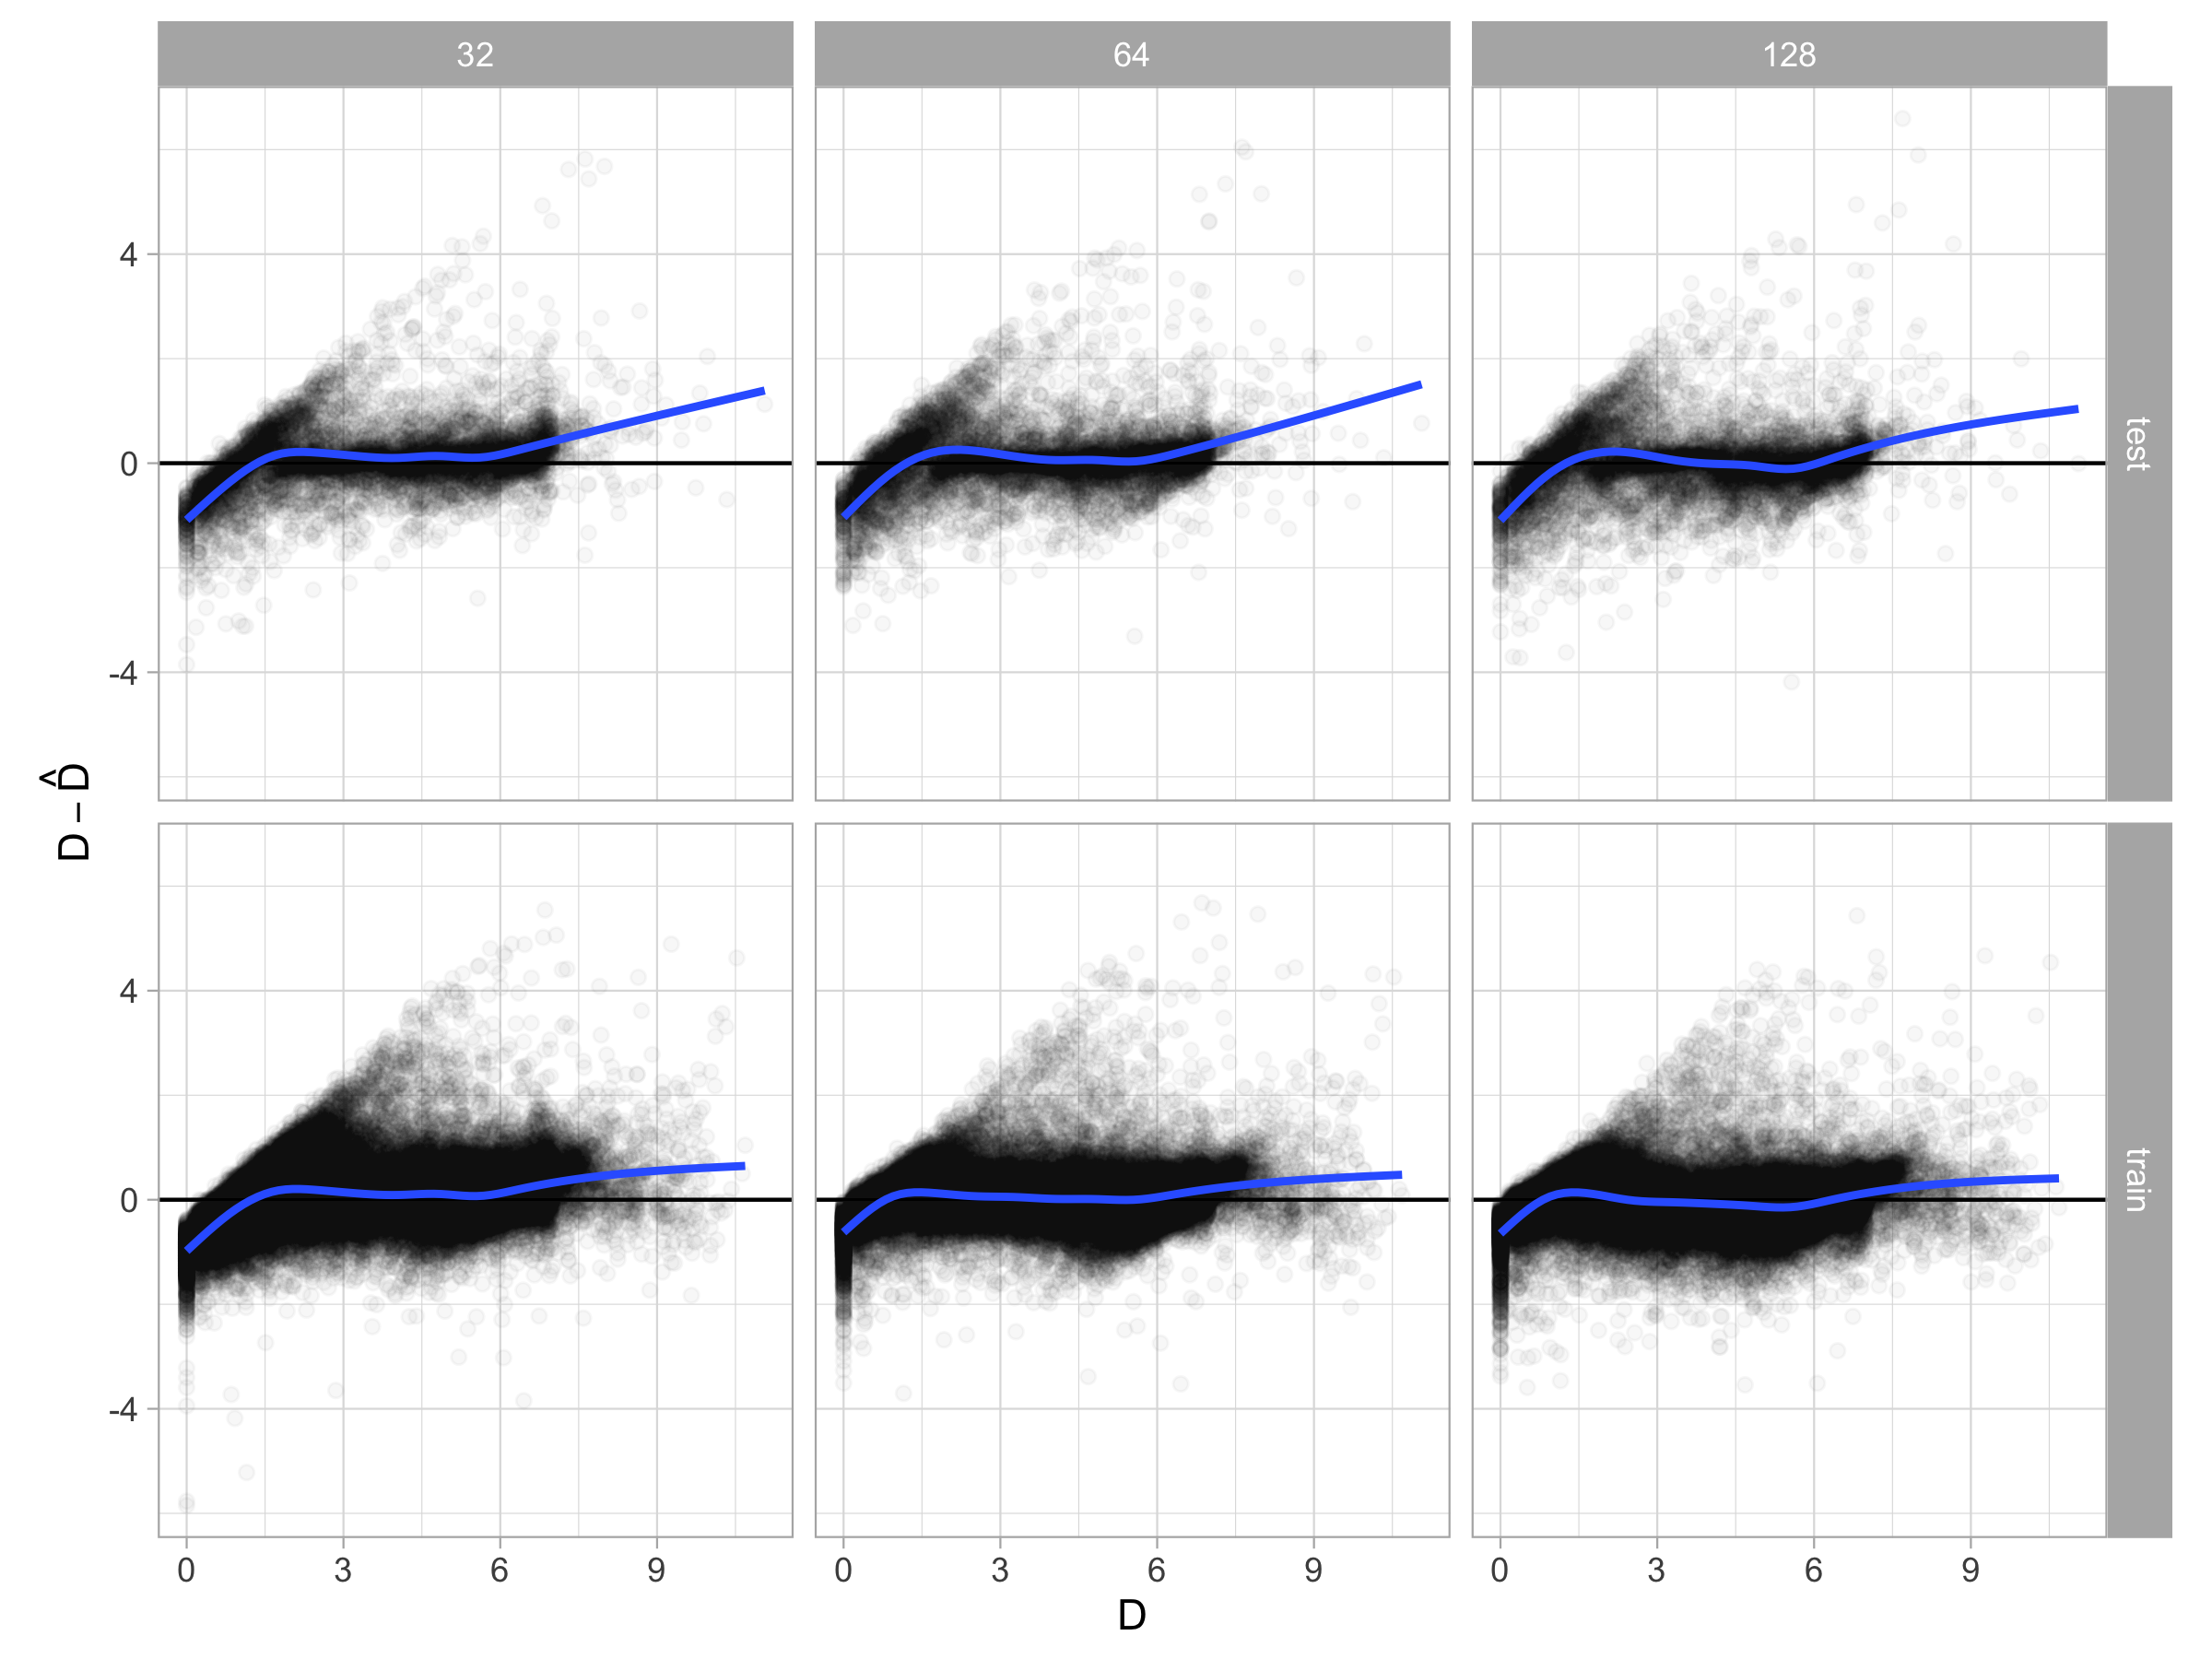
\includegraphics[width=1\linewidth]{paper_files/figure-latex/model-performance-1} 

}

\caption{Residuals vs distance plot on training and test data for three best models with different input sizes. The blue lines are smoothing curves produced by fitting gnealized additive models.}\label{fig:model-performance}
\end{figure}

\begin{figure}

{\centering 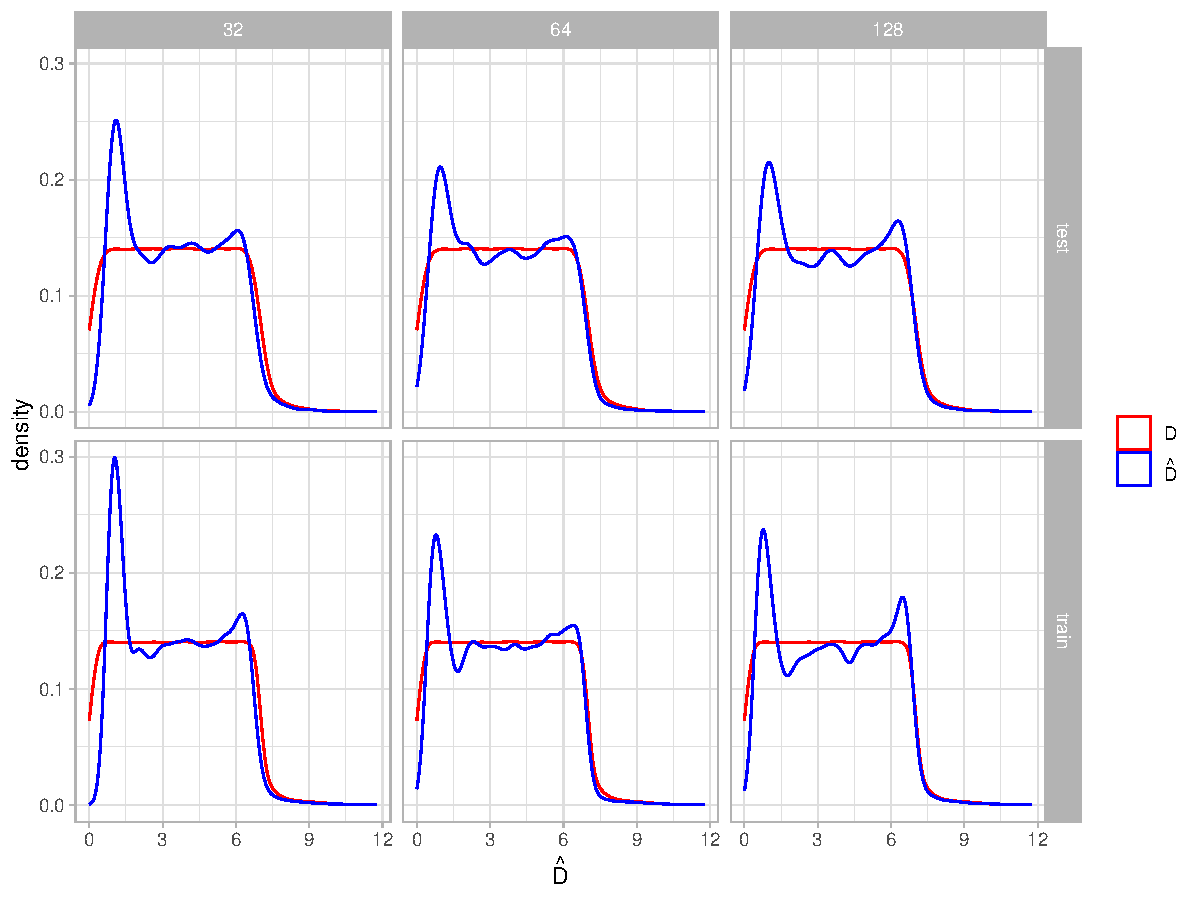
\includegraphics[width=1\linewidth]{paper_files/figure-latex/model-performance-density-1} 

}

\caption{Density plot of predicted distance on training and test data for three best models with different input sizes. The density drawn in red is the density of the distance.}\label{fig:model-performance-density}
\end{figure}

\hypertarget{comparison-with-human-visual-inference}{%
\subsection{Comparison with human visual
inference}\label{comparison-with-human-visual-inference}}

\hypertarget{overview-of-the-human-subject-experiment}{%
\subsubsection{Overview of the human subject
experiment}\label{overview-of-the-human-subject-experiment}}

\begin{itemize}
\tightlist
\item
  basic background
\item
  highlights the same and the different settings
\end{itemize}

\hypertarget{comparison}{%
\subsubsection{Comparison}\label{comparison}}

\begin{figure}

{\centering 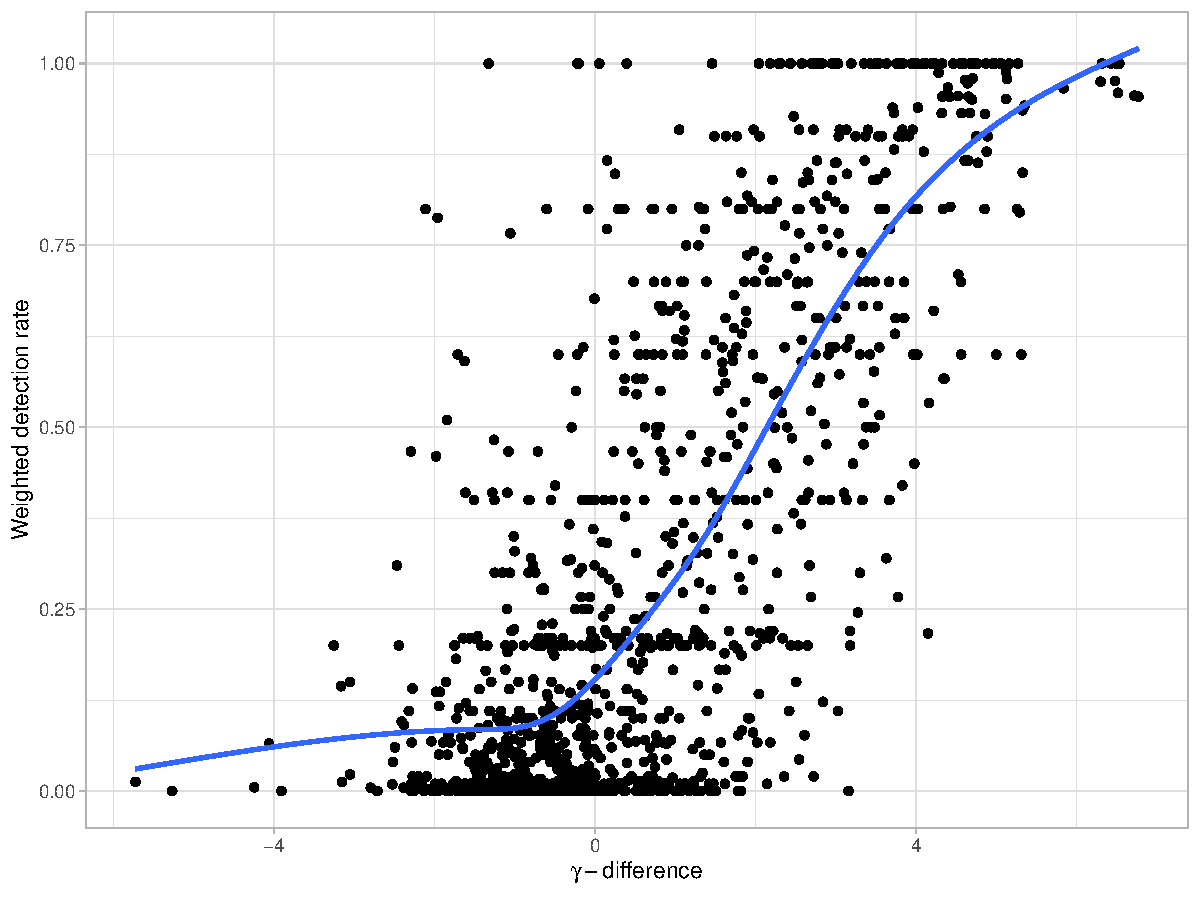
\includegraphics[width=1\linewidth]{paper_files/figure-latex/unnamed-chunk-2-1} 

}

\caption{Residuals vs distance plot on data used in the human subject experiment. The blue line is a smoothing curve produced by fitting a gnealized additive model.}\label{fig:unnamed-chunk-2}
\end{figure}

\begin{table}

\caption{\label{tab:experiment-performance}The performance of the $32 \times 32$ model on the data used in the human subject experiment.}
\centering
\begin{tabular}[t]{lllll}
\toprule
Type & RMSE & $R^2$ & MAE & Huber loss\\
\midrule
heteroskedasticity & 0.768 & 0.863 & 0.594 & 0.263\\
non-linearity & 0.731 & 0.817 & 0.560 & 0.242\\
\bottomrule
\end{tabular}
\end{table}

It can be observed from Table \ref{tab:experiment-performance} that all
the performance metrics are lower than the metrics evaluated on the test
data.

\begin{figure}

{\centering 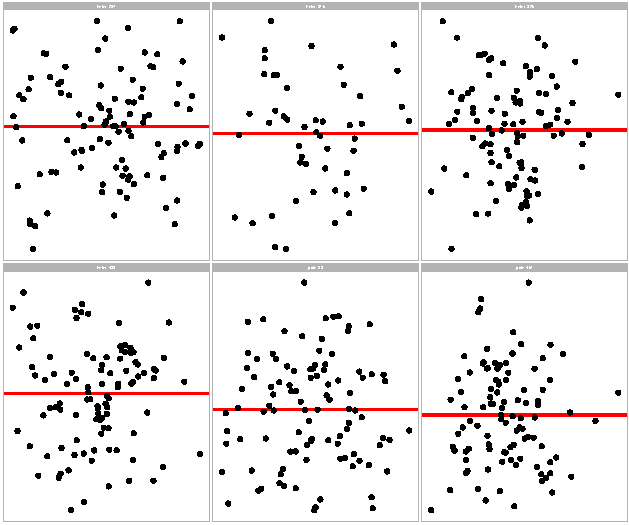
\includegraphics[width=1\linewidth]{paper_files/figure-latex/unnamed-chunk-3-1} 

}

\caption{A weighted detection rate vs $\delta$-differnence plot.}\label{fig:unnamed-chunk-3}
\end{figure}

\begin{figure}

{\centering 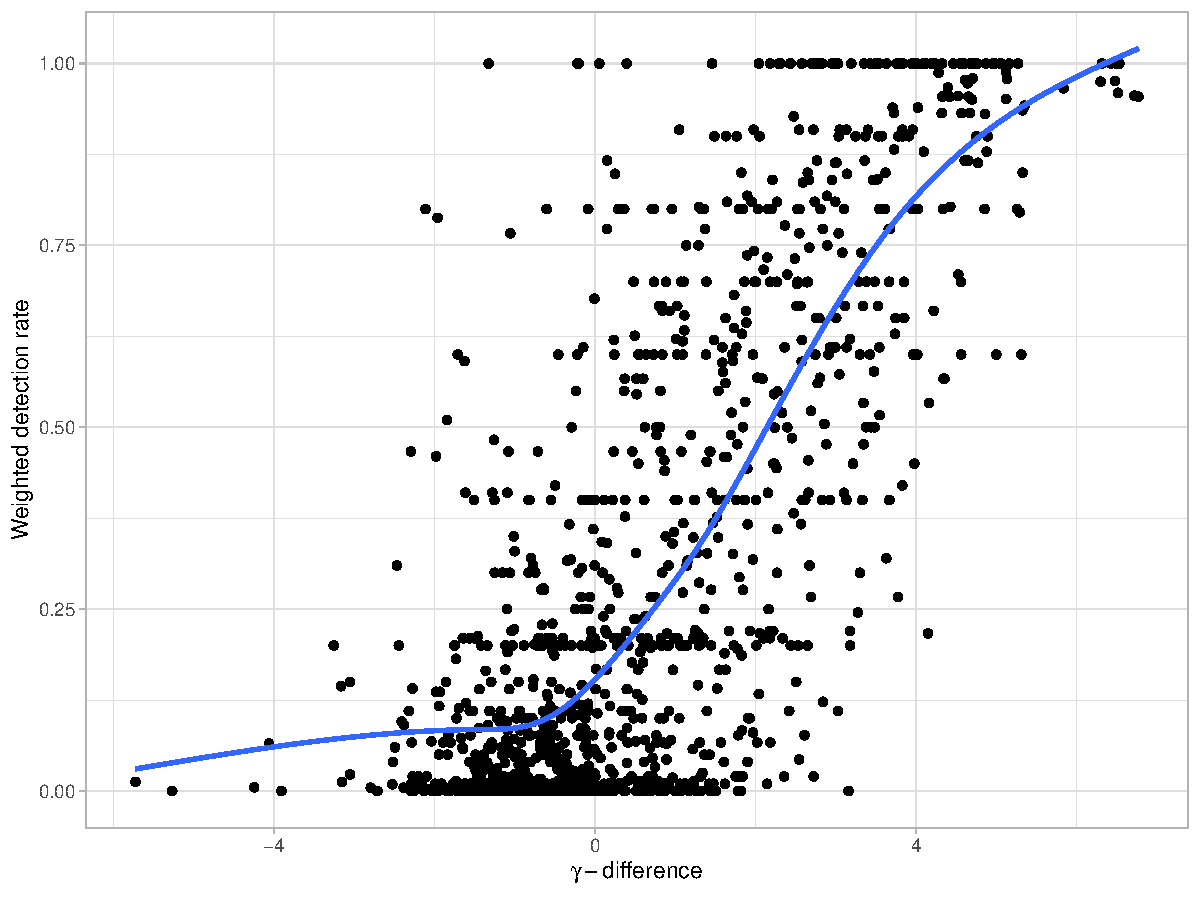
\includegraphics[width=1\linewidth]{paper_files/figure-latex/unnamed-chunk-4-1} 

}

\caption{A weighted detection rate vs $\gamma$-number of extreme nulls plot.}\label{fig:unnamed-chunk-4}
\end{figure}

\begin{figure}

{\centering 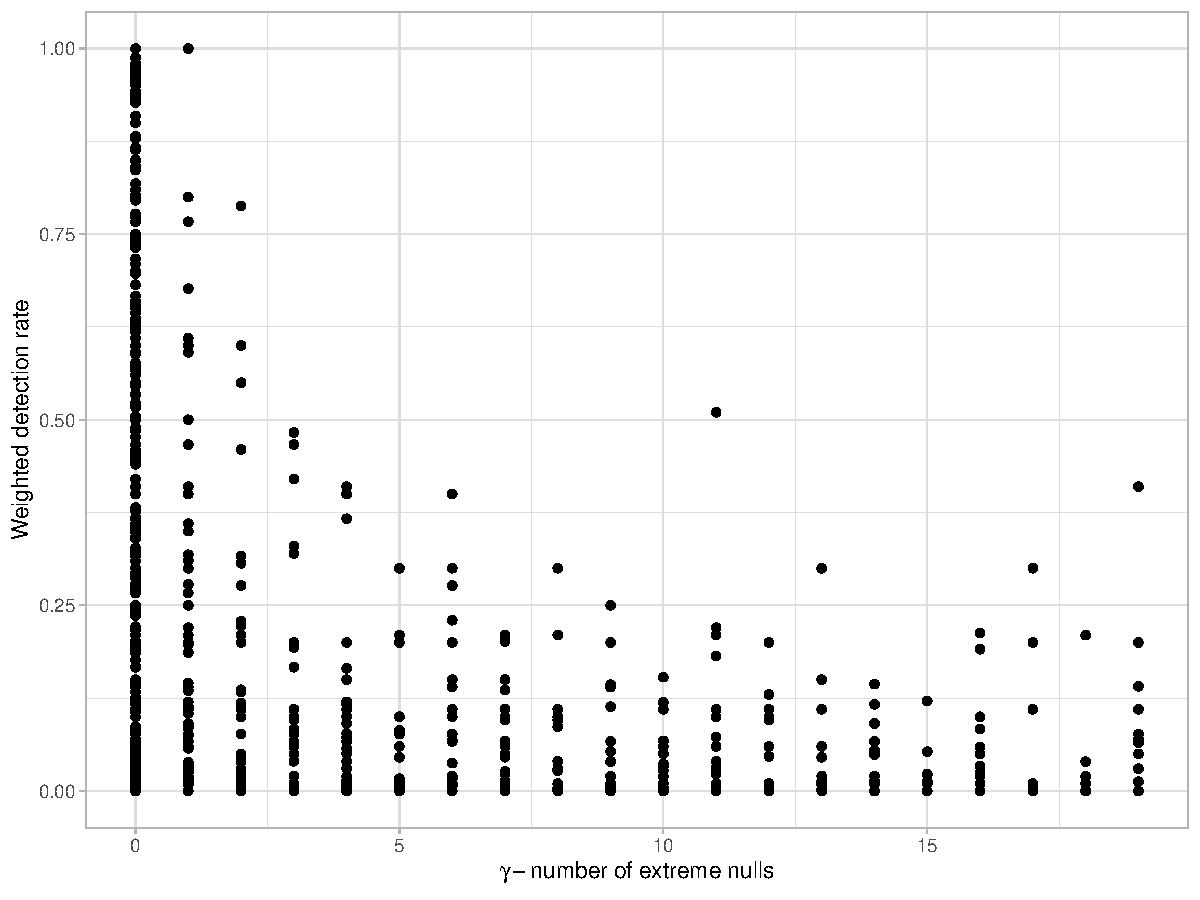
\includegraphics[width=1\linewidth]{paper_files/figure-latex/unnamed-chunk-5-1} 

}

\caption{A weighted detection rate vs $\delta$-differnence plot for lineups evaluated by 11 people.}\label{fig:unnamed-chunk-5}
\end{figure}

\begin{figure}

{\centering 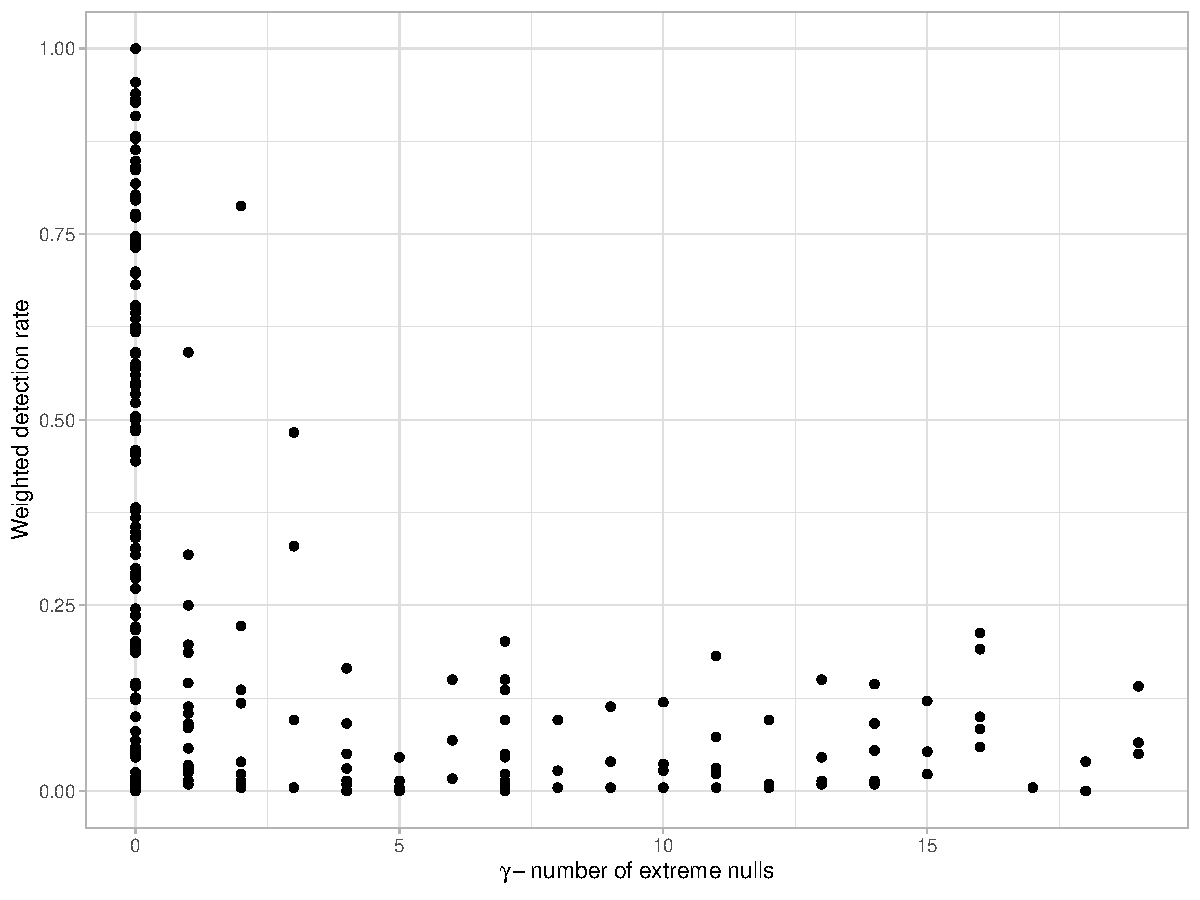
\includegraphics[width=1\linewidth]{paper_files/figure-latex/unnamed-chunk-6-1} 

}

\caption{A weighted detection rate vs $\gamma$-number of extreme nulls plot for lineups evaluated by 11 people.}\label{fig:unnamed-chunk-6}
\end{figure}

\hypertarget{when-the-model-works}{%
\subsection{When the model works}\label{when-the-model-works}}

\begin{itemize}
\tightlist
\item
  simple examples (non-linearity, heteroskedasticity, \ldots)
\item
  datasaurus
\end{itemize}

\hypertarget{when-the-model-does-not-work}{%
\subsection{When the model does not
work}\label{when-the-model-does-not-work}}

\begin{itemize}
\tightlist
\item
  human detect but model does not
\item
  cartoon residuals?
\end{itemize}

\hypertarget{workflow-how-one-use-this-model-small-showcase}{%
\subsection{Workflow: how one use this model? (small
showcase)}\label{workflow-how-one-use-this-model-small-showcase}}

\hypertarget{dicussion}{%
\section{Dicussion}\label{dicussion}}

There are other kinds of residual departures like autocorrelation that
are not considered in this study. The primary goal of this paper is to
establish a new way of evaluating residual plot and conducting visual
test with computer vision models. Building computer vision models for
other model violations and other types of diagnostic plots could be
future directions of this field.

\hypertarget{conclusion}{%
\section{Conclusion}\label{conclusion}}

\begin{itemize}
\tightlist
\item
  Summary of findings
\item
  Contributions to the field
\item
  Future directions for research
\end{itemize}

\bibliographystyle{tfcad}
\bibliography{ref.bib}





\end{document}
